\chapter{Results of the H2Mu search} \label{chp:hmm_results}

The analysis in the VH category is combined with those in the \ggH, \qqH, and \ttH categories~\cite{Sirunyan_2021}.
All results and plots in this chapter are published in Ref.~\cite{Sirunyan_2021}.
In this combined analysis, the mass of the Higgs boson is expected at \mh = 125.38~\GeV~\cite{2020135425},
which is the most precise measurement of the Higgs boson mass up to date.
Figure~\ref{fig:sum_cats_comp} summarizes the expected signal composition in all subcategories of the \hmm analysis.
Figure~\ref{fig:sum_cats_SB} summarizes the expected $S/(S+B)$ and $S/\sqrt{B}$ in all subcategories,
in which the signal and background yields are calculated by integrating the expectations within the FWHM range of the signal peak for the \ggH, \VH, and \ttH subcategories,
while for the \qqH category the considered mass range is $115~\GeV < \mmm < 135~\GeV$.

\begin{figure*}[!htb]
    \centering
    \captionsetup{justification=justified}
    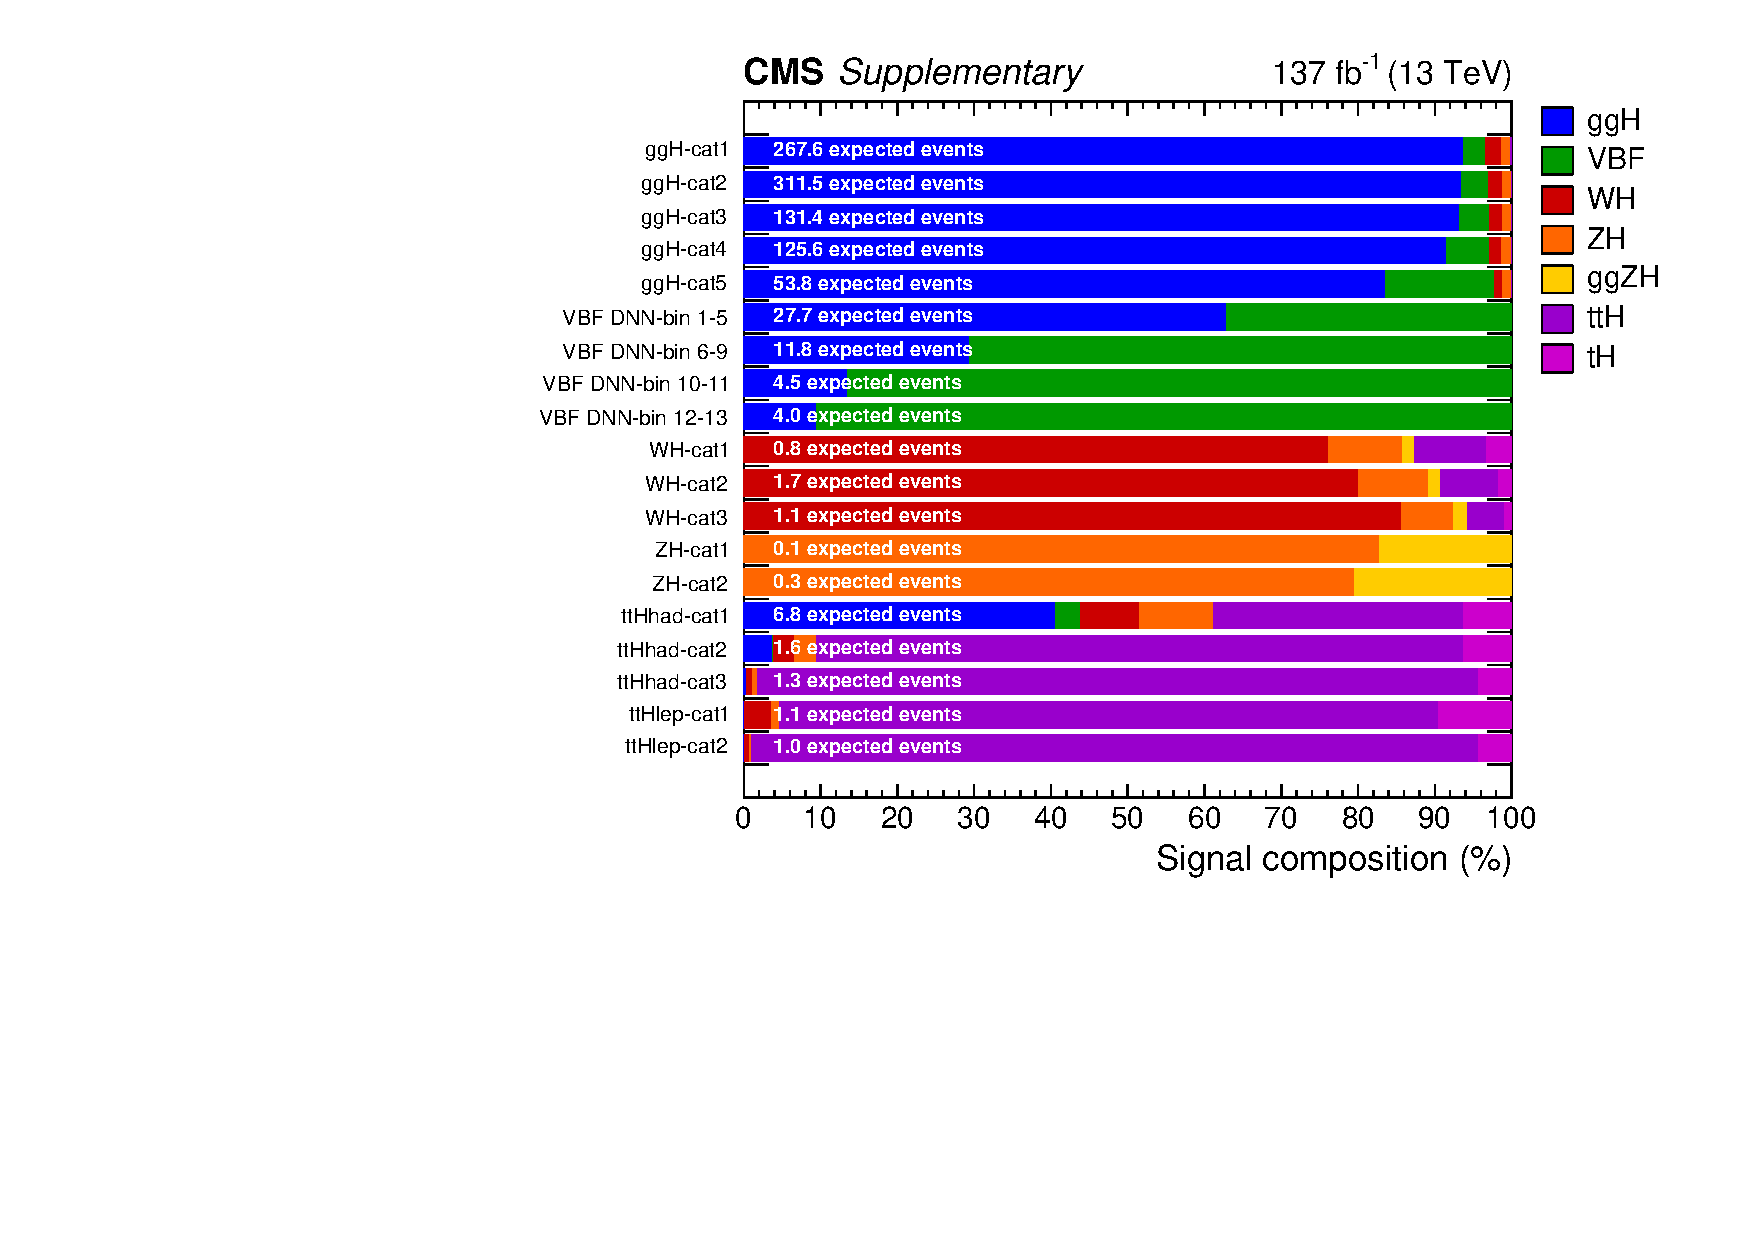
\includegraphics[width=0.80\textwidth]{pics/results/sig_composition.pdf}
    \caption{Expected fraction of signal events per production mode in the different subcategories for \mh = 125.38~\GeV.
             The tH contribution is defined as the sum of \tHq and \tHW processes.}
    \label{fig:sum_cats_comp}
\end{figure*}

\begin{figure*}[!htb]
    \centering
    \captionsetup{justification=justified}
    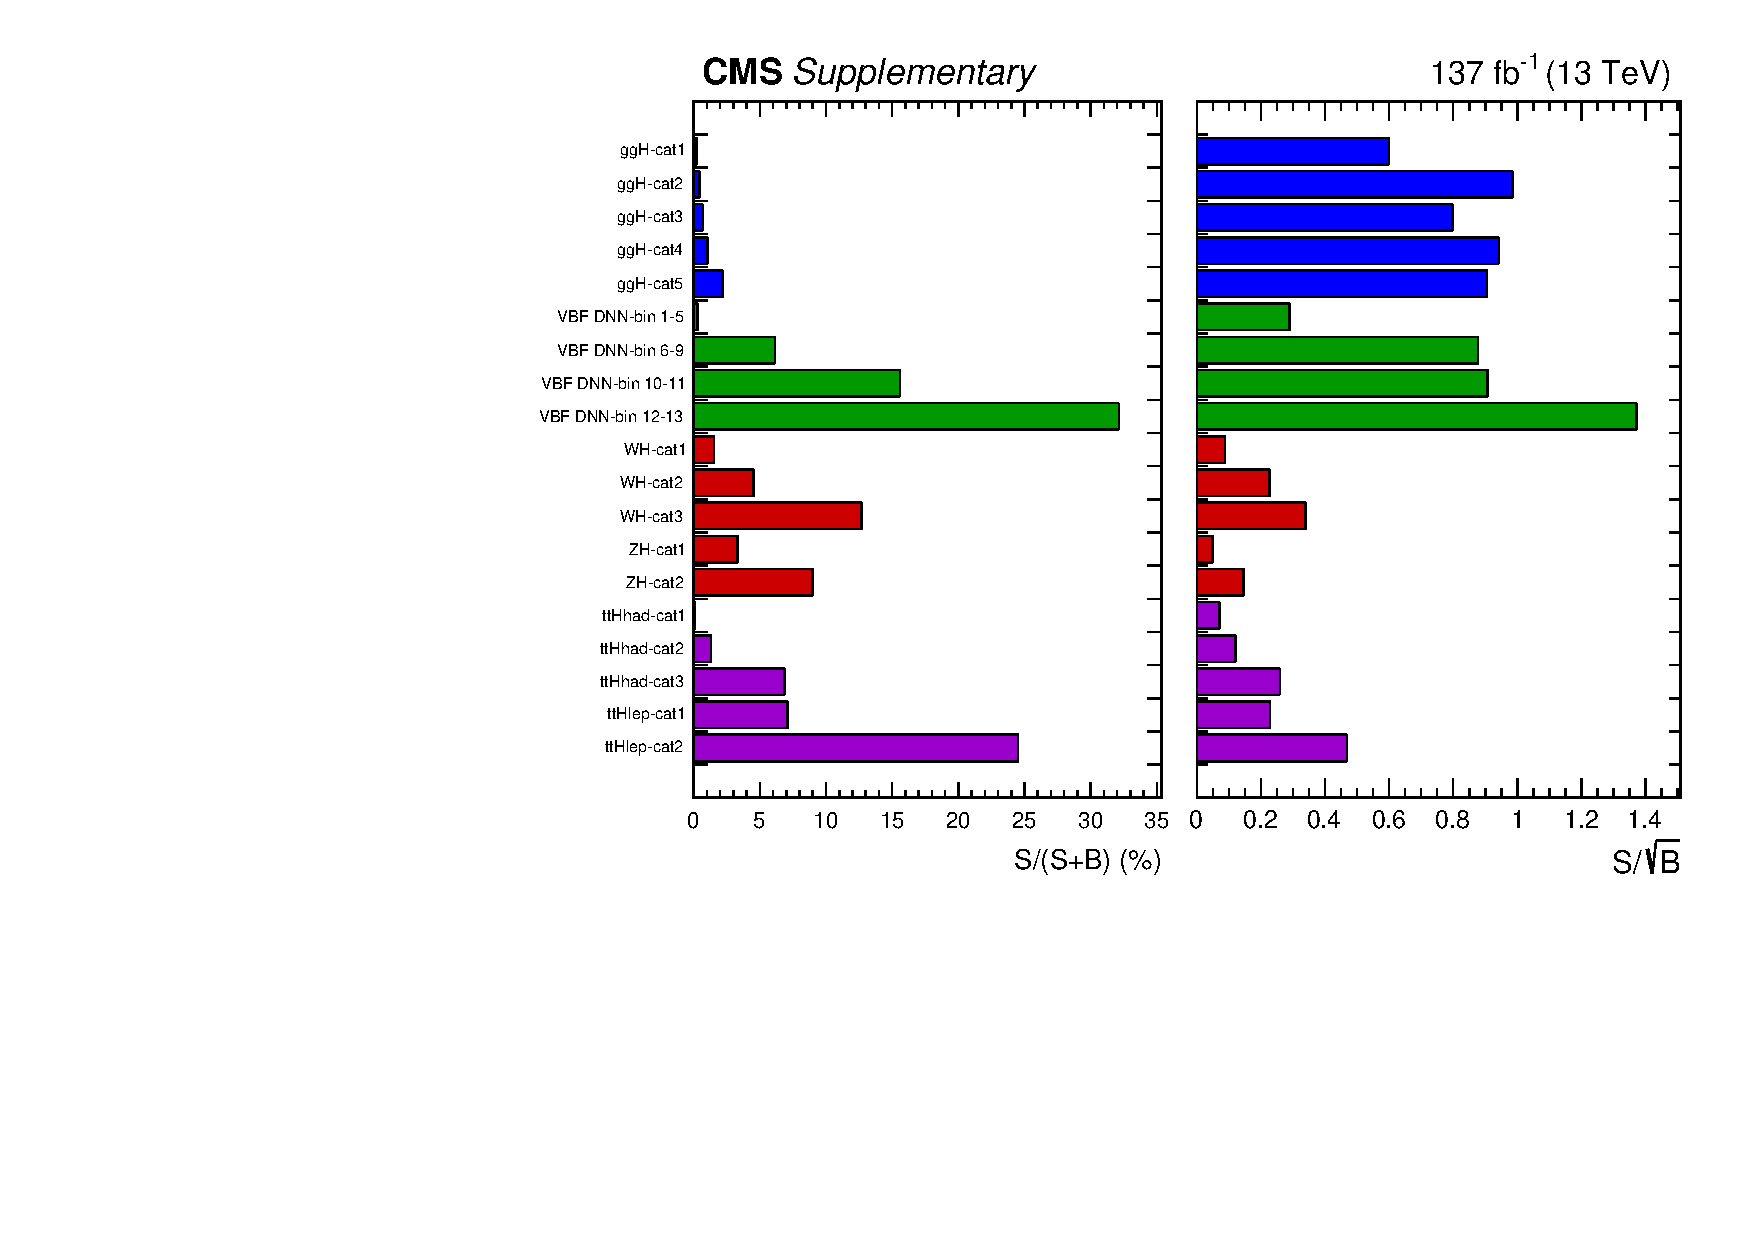
\includegraphics[width=0.80\textwidth]{pics/results/purity_signif.pdf}
    \caption{Expected $S/(S+B)$ and $S/\sqrt{B}$ in different subcategories, 
             where $S$ and $B$ indicate the number of expect signal and background events, respectively.}
    \label{fig:sum_cats_SB}
\end{figure*}


\begin{figure*}[!htb]
    \centering
    \captionsetup{justification=justified}
    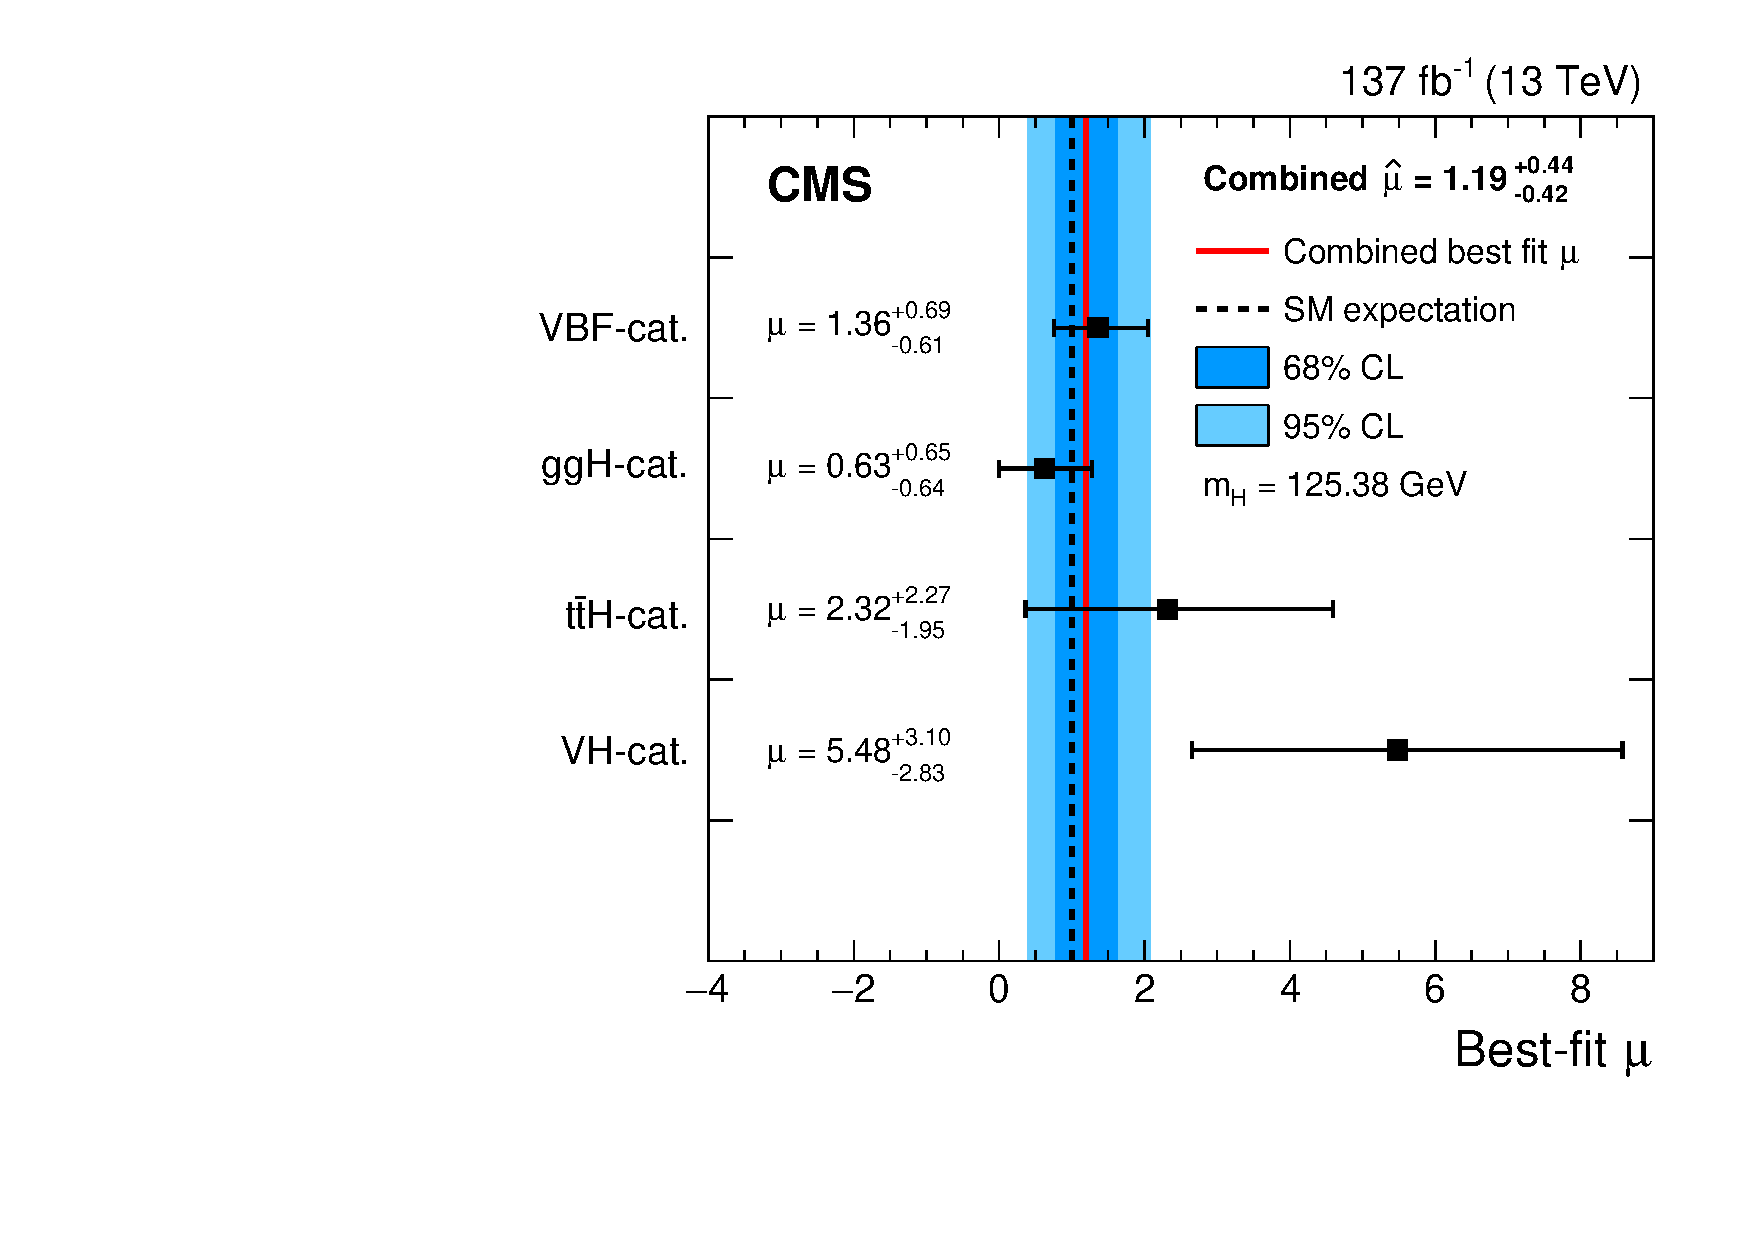
\includegraphics[width=0.60\textwidth]{pics/results/sig_strength.pdf}
    \caption{Signal strength modifiers measured for \mh = 125.38~\GeV in each production category (black points) 
             are compared to the result of the combined fit (solid red line) and the SM expectation (dashed gray line).}
    \label{fig:sum_sig_strength}
\end{figure*}

Maximum-likelihood fits are performed in each category following the strategies explained in Chapter~\ref{chp:hmm_overview}:
analytic \mmm shape fits for \ggH, \ttH, and \VH categories, and template DNN shape fit for the \qqH category.
The individual signal strength modifier from each category is summarized in Figure~\ref{fig:sum_sig_strength},
with the Higgs signal expected at \mh = 125.38~\GeV.
A combined fit is performed across all categories with one common signal strength modifier, 
whose best fit value is $\hat{\mu} = 1.19^{+0.41}_{-0.40} \text{(stat)}^{+0.17}_{-0.16} \text{(syst)}$.
Figure~\ref{fig:sum_mass_shape} shows the \mmm distribution for the weighted combination of all categories.
Please note that this plot is only for illustration, as the \qqH result is obtained by fitting DNN shapes not the \mmm shape.
In Figure~\ref{fig:sum_mass_shape}, \ggH, \ttH, and \VH subcategories are weighted by their $S/(S+B)$ ratios.
For the \qqH category, a mass-decorrelated DNN is obtained by setting the \mmm value for all events to 125~\GeV,
and a per-event $S/(S+B)$ weight is calculated based on this mass-decorrelated DNN output. 
This weight is applied to the \qqH \mmm distribution, 
in which all nuisance parameters and the signal strength are set to their post-fit values from the actual DNN fit.
A clear excess of events is seen around 125~\GeV in the background-subtracted distribution in the lower panel.

\begin{figure*}[!htb]
    \centering
    \captionsetup{justification=justified}
    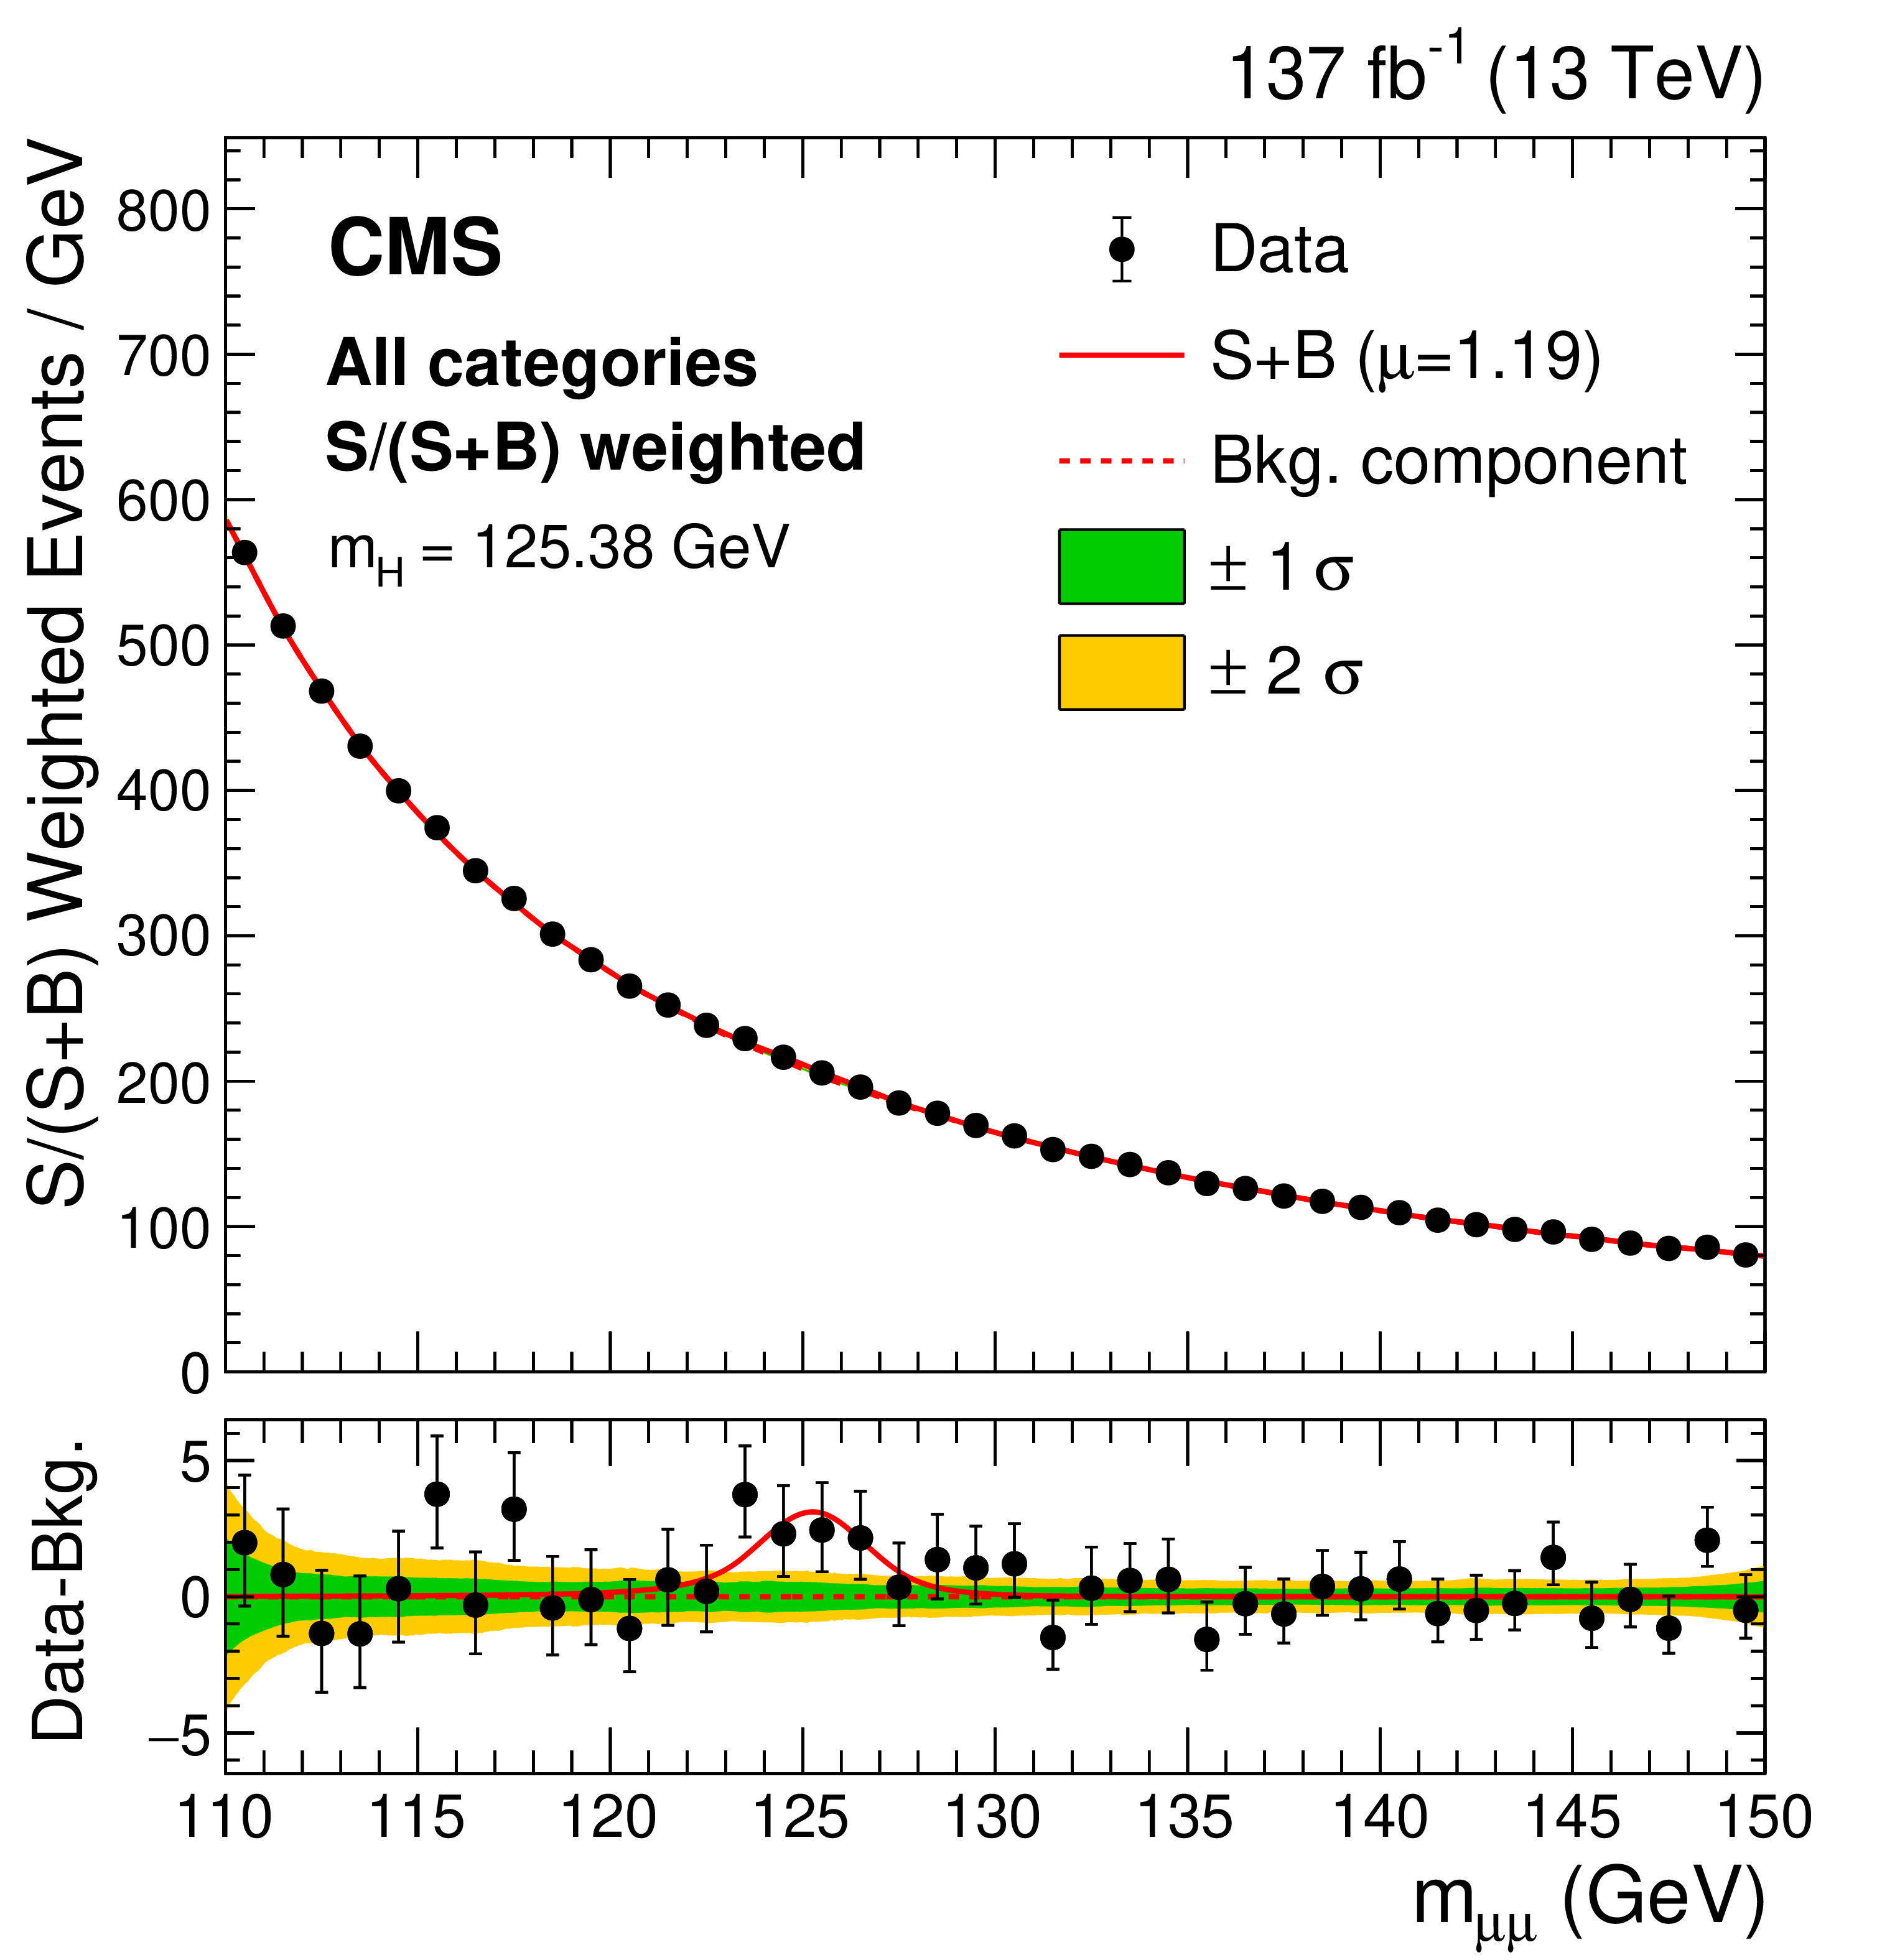
\includegraphics[width=0.60\textwidth]{pics/results/sum_mass_dist.png}
    \caption{Post-fit \mmm distribution of the weighted combination of all categories.
             Subcategories are weighted proportionally to $S/(S+B)$ ratio. 
             The lower panel in the plots shows the residual distribution after background subtraction.
             The green and yellow bands show the one and two standard deviation of the background component uncertainty.}
    \label{fig:sum_mass_shape}
\end{figure*}


The statistical uncertainty is determined by performing a likelihood scan of $\mu$ with all nuisance parameters fixed at their best fit values.
And the systematic uncertainty is calculated as the difference in quadrature between the total uncertainty and the statistical component.
This result makes the most precise measurement of the \hmm decay rate up to date.
Assuming SM production cross sections for all Higgs production modes, 
the \hmm branching ratio is constrained at 95\% CL to be within $0.8 \times 10^{-4} < \brhmm < 4.5 \times 10^{-4}$.

\begin{figure*}[!htb]
    \centering
    \captionsetup{justification=justified}
    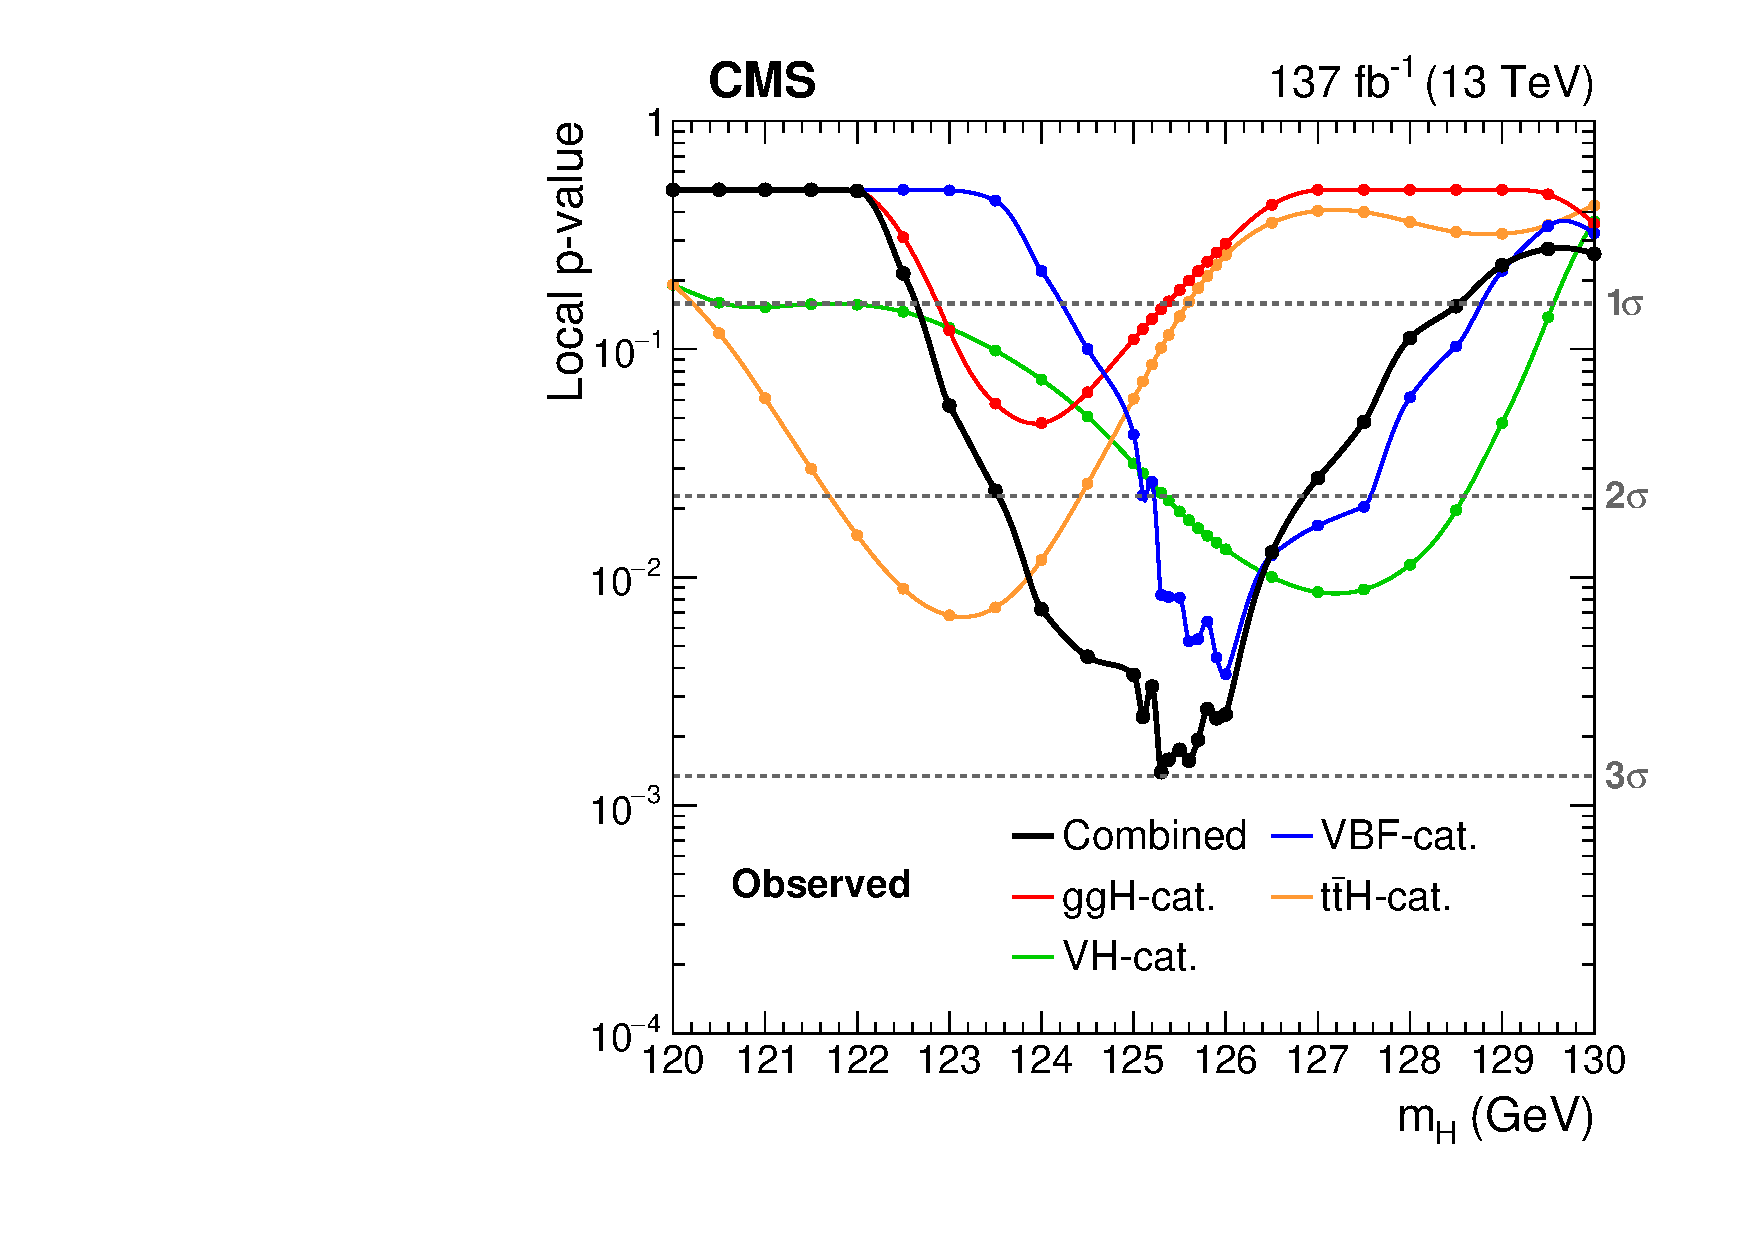
\includegraphics[width=0.45\textwidth]{pics/results/p-value_obs.pdf}
    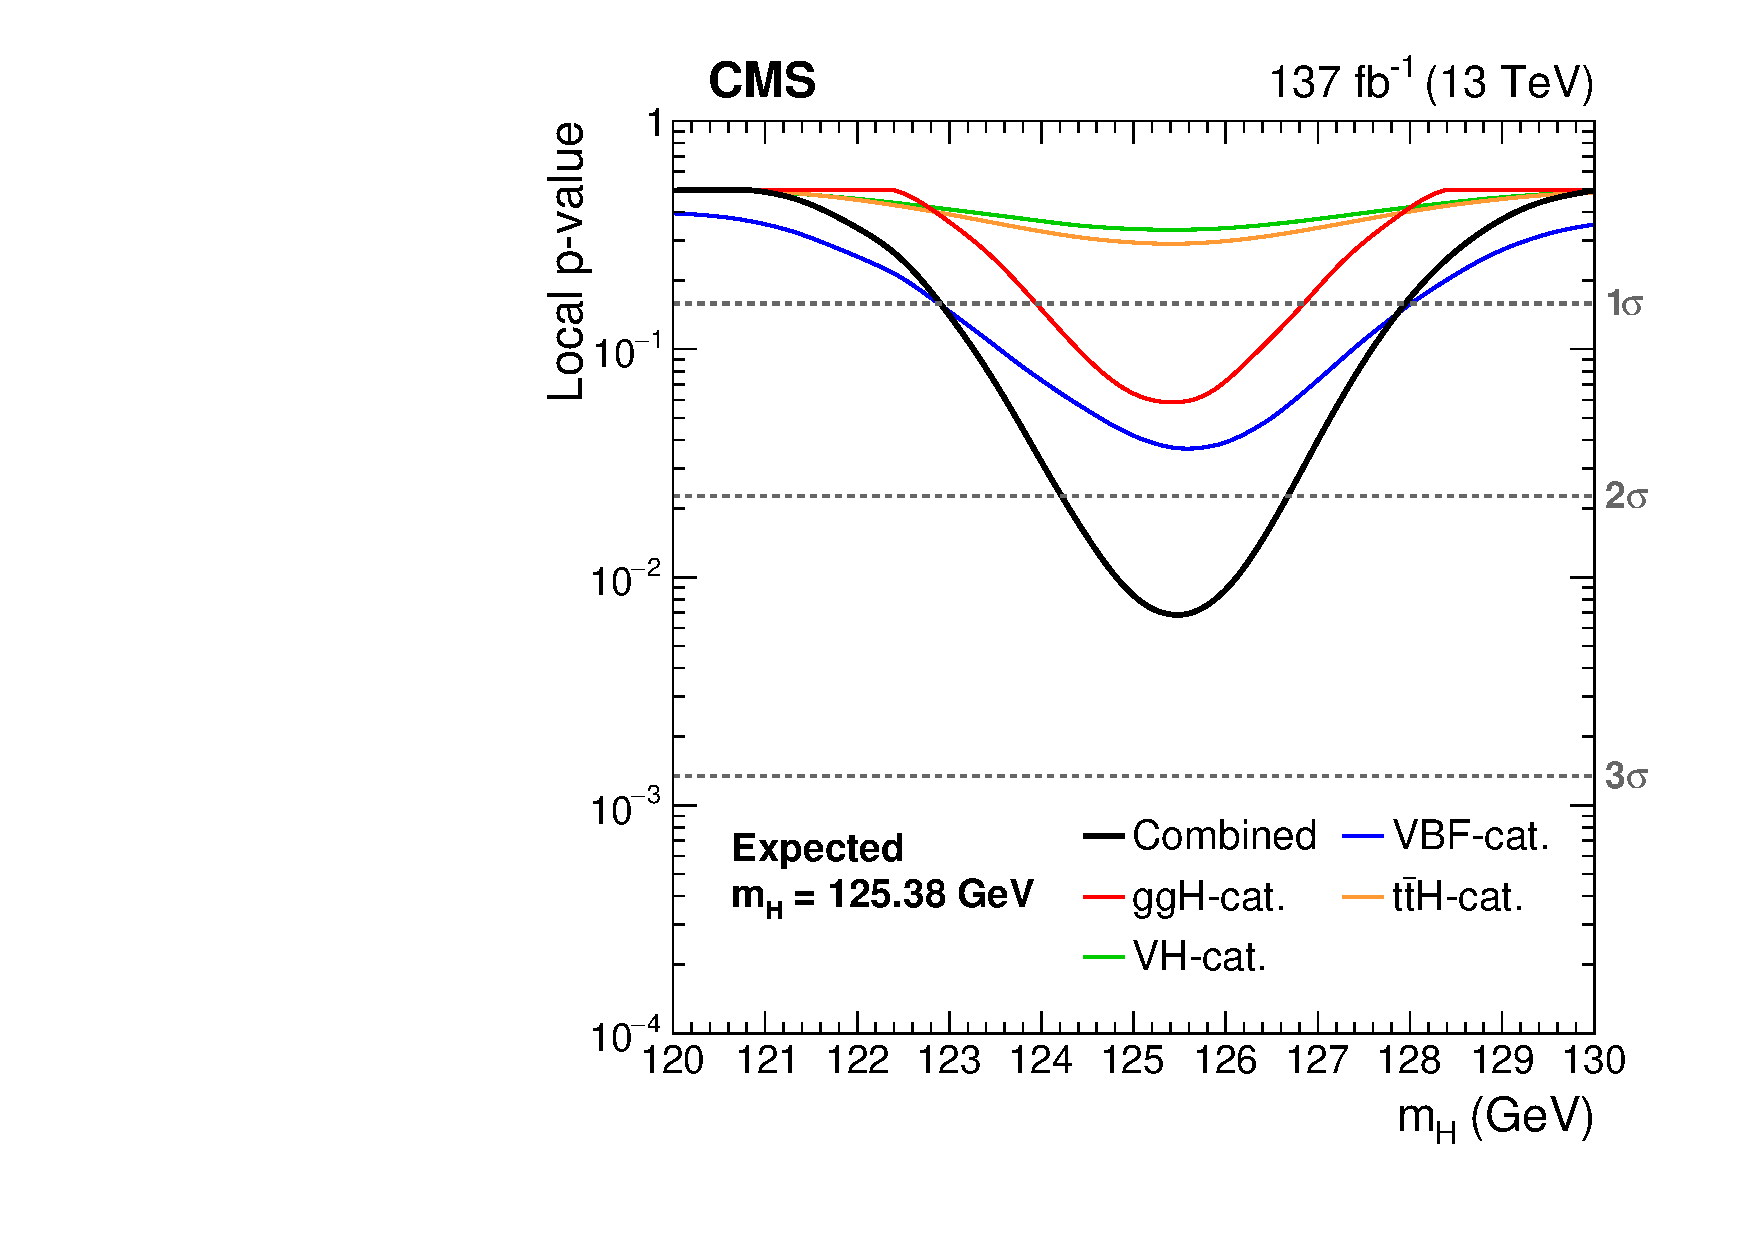
\includegraphics[width=0.45\textwidth]{pics/results/p-value_exp.pdf}
    \caption{The local p-values as a function of different \mh hypotheses, 
             for each individual categories as well as the overall combination.
             The left plot shows the observed p-values, 
             each solid marker indicating a mass point, for which the observed p-values are computed.
             The right plot shows the expected p-values calculated using the background estimate from the S+B fit 
             and injecting a signal with \mh = 125.38~\GeV and $\mu = 1$.}
    \label{fig:p_value_scan}
\end{figure*}

The statistical significance of a signal presence is tested against the null hypothesis,
in which no signal is assumed and the observed distribution is purely raised by statistical fluctuation in background.
The local $p$-value quantifies the probability for the background to produce such a fluctuation larger than the apparent signal observed in the search region.
A scan of $p$-value is performed across the mass range of $120~\GeV< \mh < 130~\GeV$.
Figure~\ref{fig:p_value_scan} shows the observed and expected $p$-values for individual categories as well as the overall combination.
The expected $p$-values are calculated with a SM signal at 125.38~\GeV injected on top of the background expectation.
The observed (expected for $\mu = 1$) significance at \mh = 125.38~\GeV of the incompatibility with the background-only hypothesis is 3.0~(2.5) standard deviations,
while the observed (expected for $\mu = 0$) upper limit of the signal strength at the 95\% confidence level is 1.9~(0.8) times the SM expectation.
This result establishes the first evidence of the Higgs boson decay to fermions of the second generation. 

\begin{figure*}[!htb]
    \centering
    \captionsetup{justification=justified}
    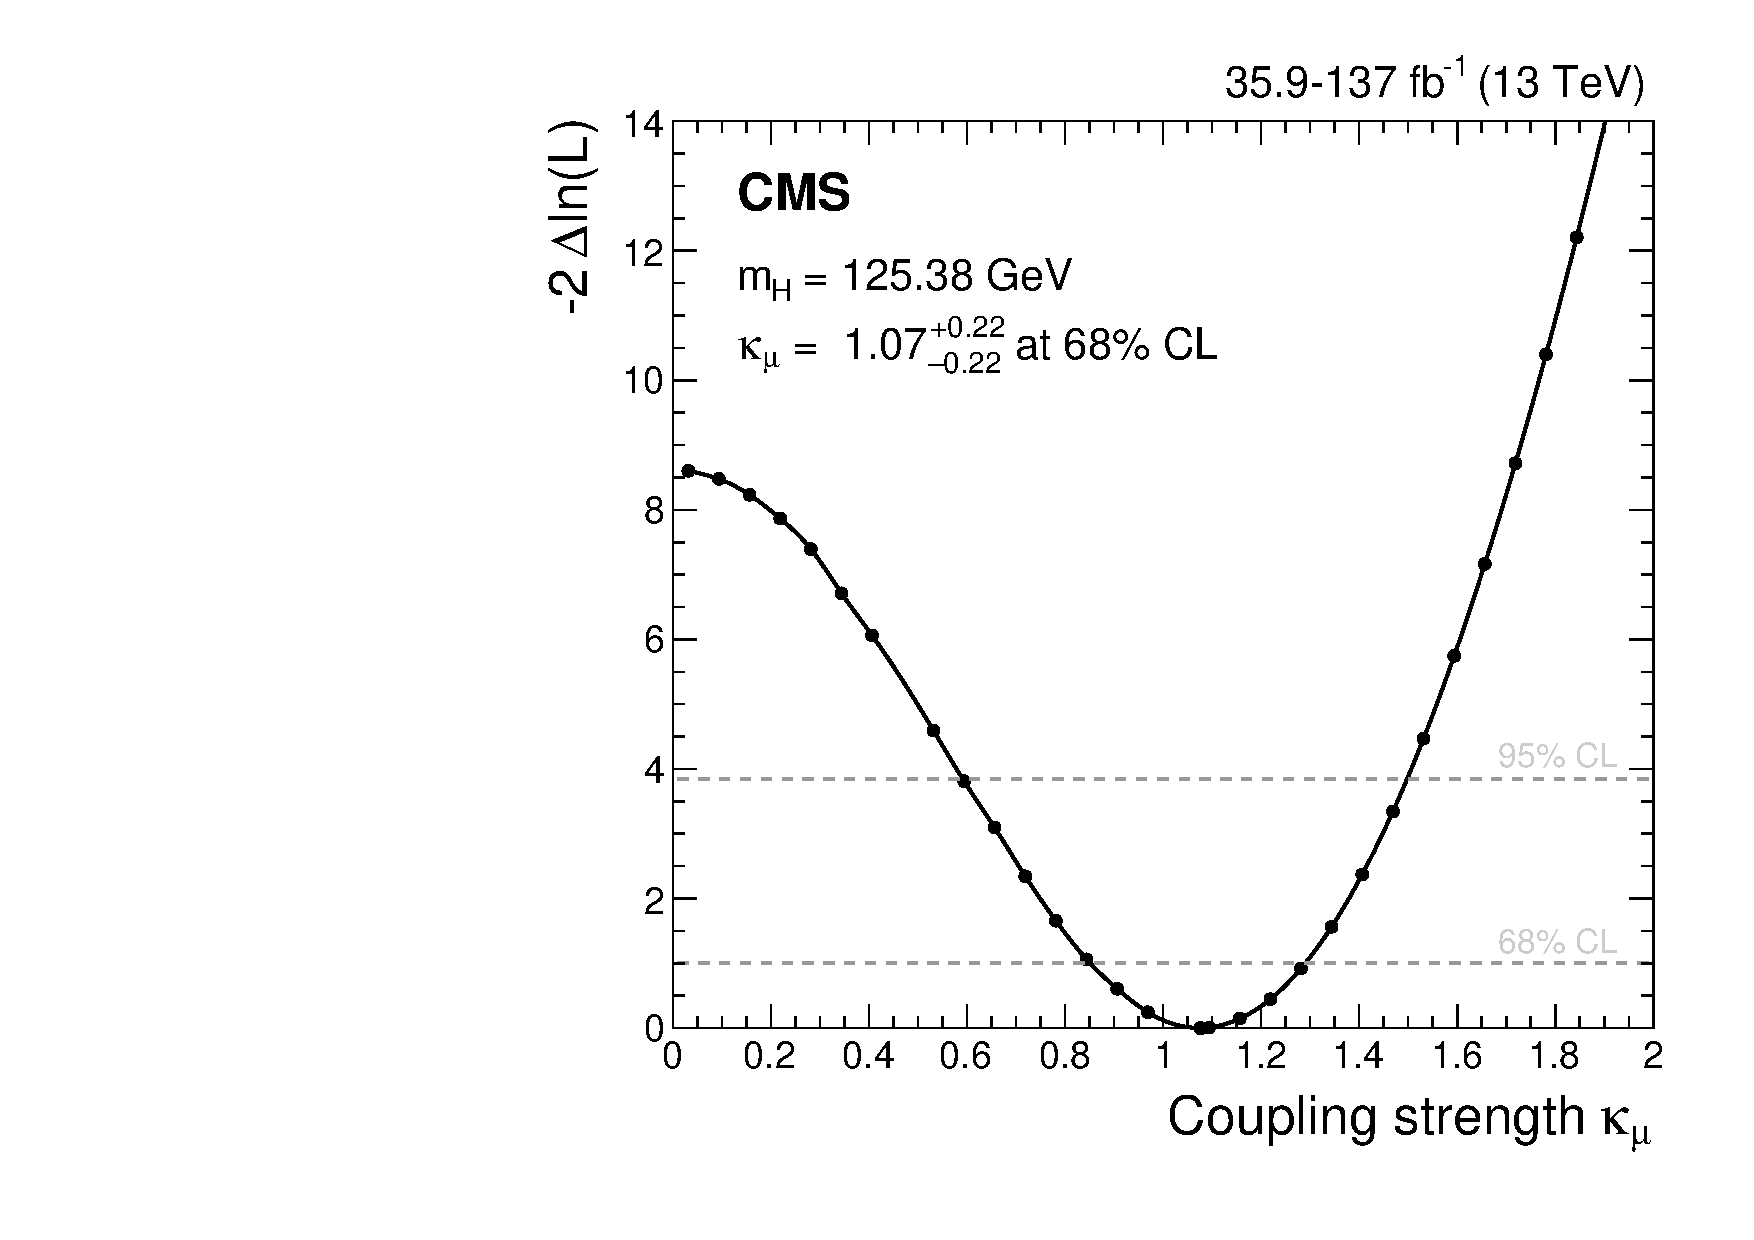
\includegraphics[width=0.60\textwidth]{pics/results/kappa_mu.pdf}
    \caption{The observed profile likelihood ratio as a function of $\kappa_{\mu}$ for \mh = 125.38~\GeV.}
    \label{fig:kappa_scan}
\end{figure*}

\begin{figure*}[!htb]
    \centering
    \captionsetup{justification=justified}
    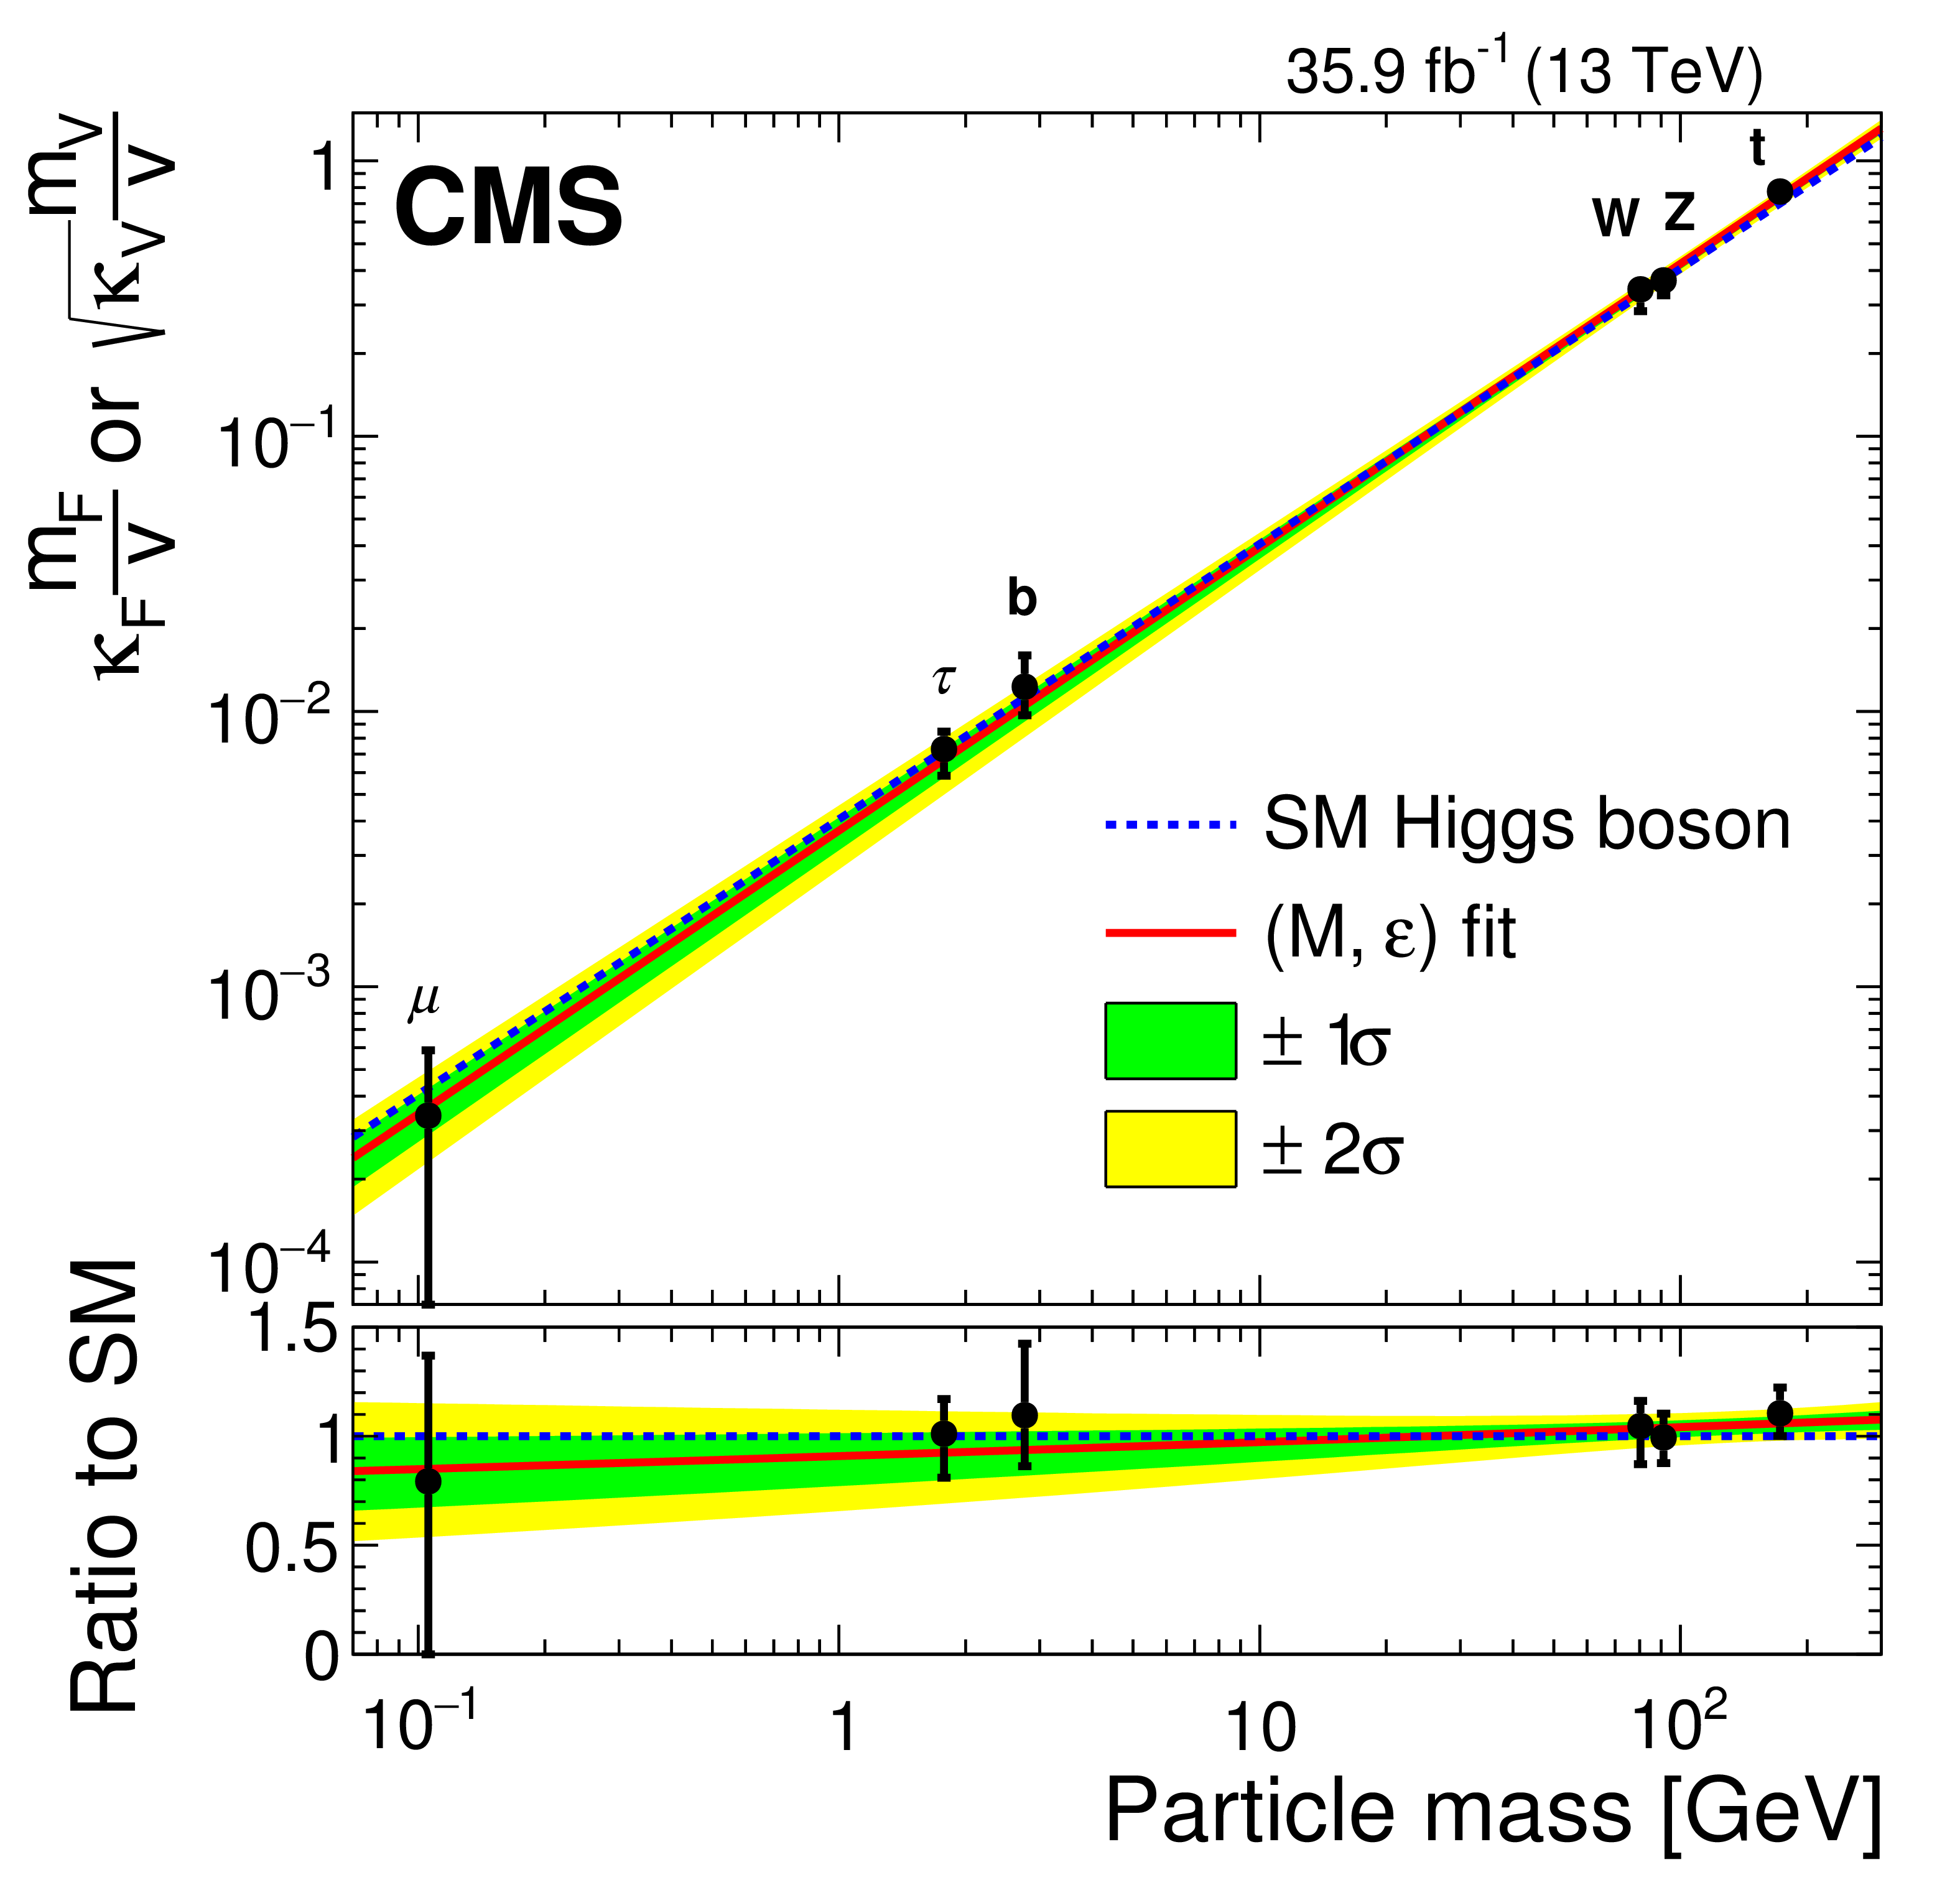
\includegraphics[width=0.45\textwidth]{pics/Intro/higgs_coupling_2016.png}
    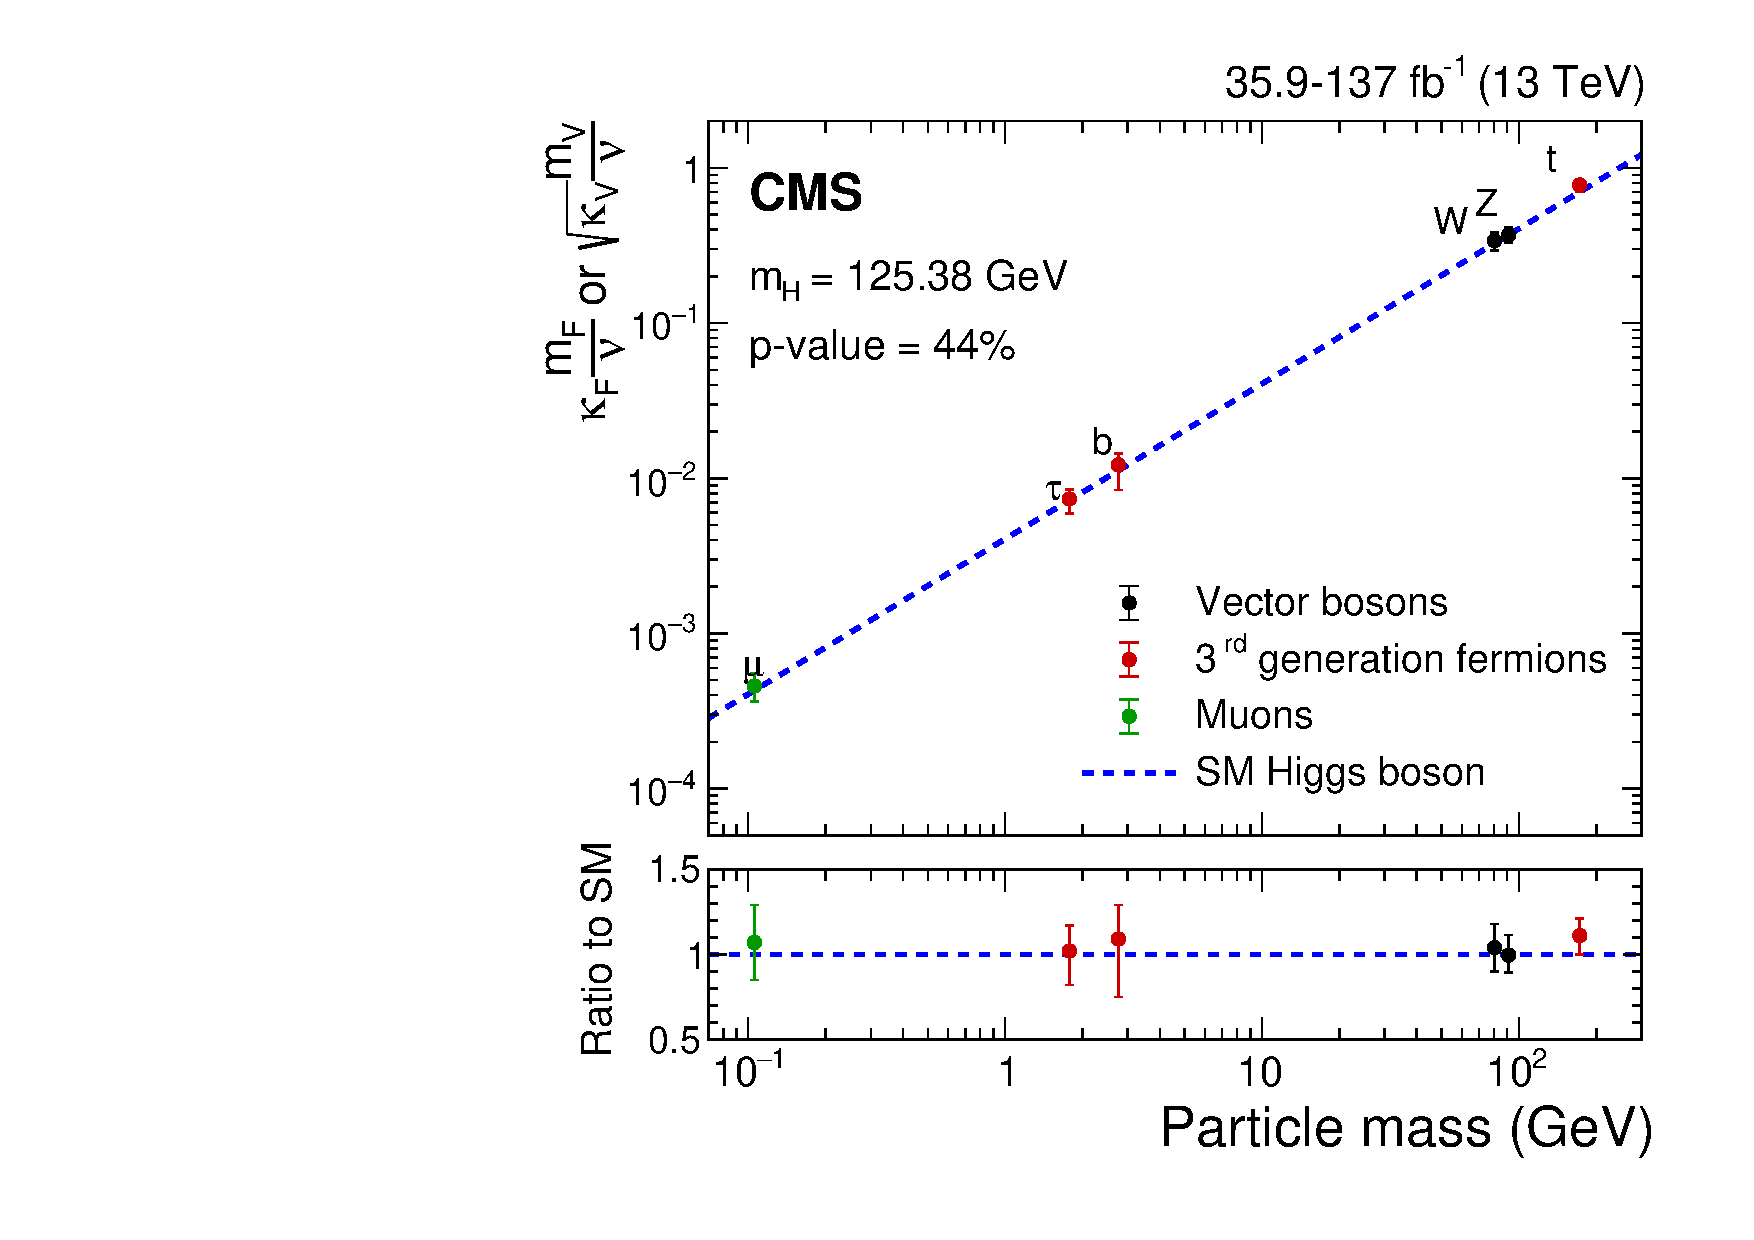
\includegraphics[width=0.45\textwidth]{pics/results/higgs_coupling_new.pdf}
    \caption{Left: A duplicate of Figure~\ref{fig:higgs_2016}, taken from Ref.~\cite{Sirunyan:2640611}. 
             Summary of the CMS measurements on the Higgs coupling to fermions and bosons based on data recorded in 2016.
             Right: The coupling strength measurements updated with this \hmm result.}
    \label{fig:higgs_coupling_new}
\end{figure*}

Finally, as discussed in Section~\ref{sec:SM_parameters}, the coupling strength between the Higgs boson and the muon is an essential parameter to SM.
This work also provides the best constraint on the Higgs-muon coupling up to date.
The signal strength of \hmm decay cannot be translated directly into a measurement of the Higgs boson coupling to muons,
as the \hmm decay ratio is determined by all possible Higgs decays.
Assuming the Higgs boson does not decay to unknown particles, 
the Higgs coupling strengths in SM are evaluated in the $\kappa$-framework \cite{Heinemeyer:2013tqa}.
The measurement of Higgs coupling strengths is performed by combining many Higgs analyses,
and the latest measurement by CMS~\cite{Sirunyan:2640611} prior to this work is based on collision data at $\sqrt{s} = 13~\TeV$ recorded in 2016, corresponding to an integrated luminosity of 35.9~\invfb.
This \hmm analysis is combined with Ref.~\cite{Sirunyan:2640611}, updating the coupling strengths measurement.
The likelihood scan of $\kappa_{\mu}$ is shown in Figure~\ref{fig:kappa_scan}.
The best fit value for $\kappa_{\mu}$ is 1.07 and the corresponding observed 68\% confidence interval is $0.85 < \kappa_{\mu} < 1.29$.
The global result of all coupling modifiers is shown in Figure~\ref{fig:higgs_coupling_new}, updating Figure~\ref{fig:higgs_2016}.

In summary, an analysis on the \hmm decay is performed with $pp$ collision data at $\sqrt{s} = 13~\TeV$ collected by CMS, corresponding to an integrated luminosity of 137~\invfb.
An excess of events over background-only expectation is observed (expected) with a significance of 3.0~(2.5) standard deviations for the SM Higgs boson at 125.38~\GeV. 
The measured signal strength, relative to the SM expectation, is $1.19^{+0.41}_{-0.40} \text{(stat)}^{+0.17}_{-0.16} \text{(syst)}$.
This result makes the first evidence for the decay of the Higgs boson to second generation fermions and provides the most precise measurement of the Higgs boson coupling to muons up to date. 
